After having completed the modelling and controller design for both bicycles, the final designs could then be tested on the real-world system. Firstly, the Lego prototype implementation was investigated, since it is much easier to assemble and to test in a confined space. The Lego prototype is depicted in Figure \ref{fig:lego} below.

\begin{figure}[H]
\centering
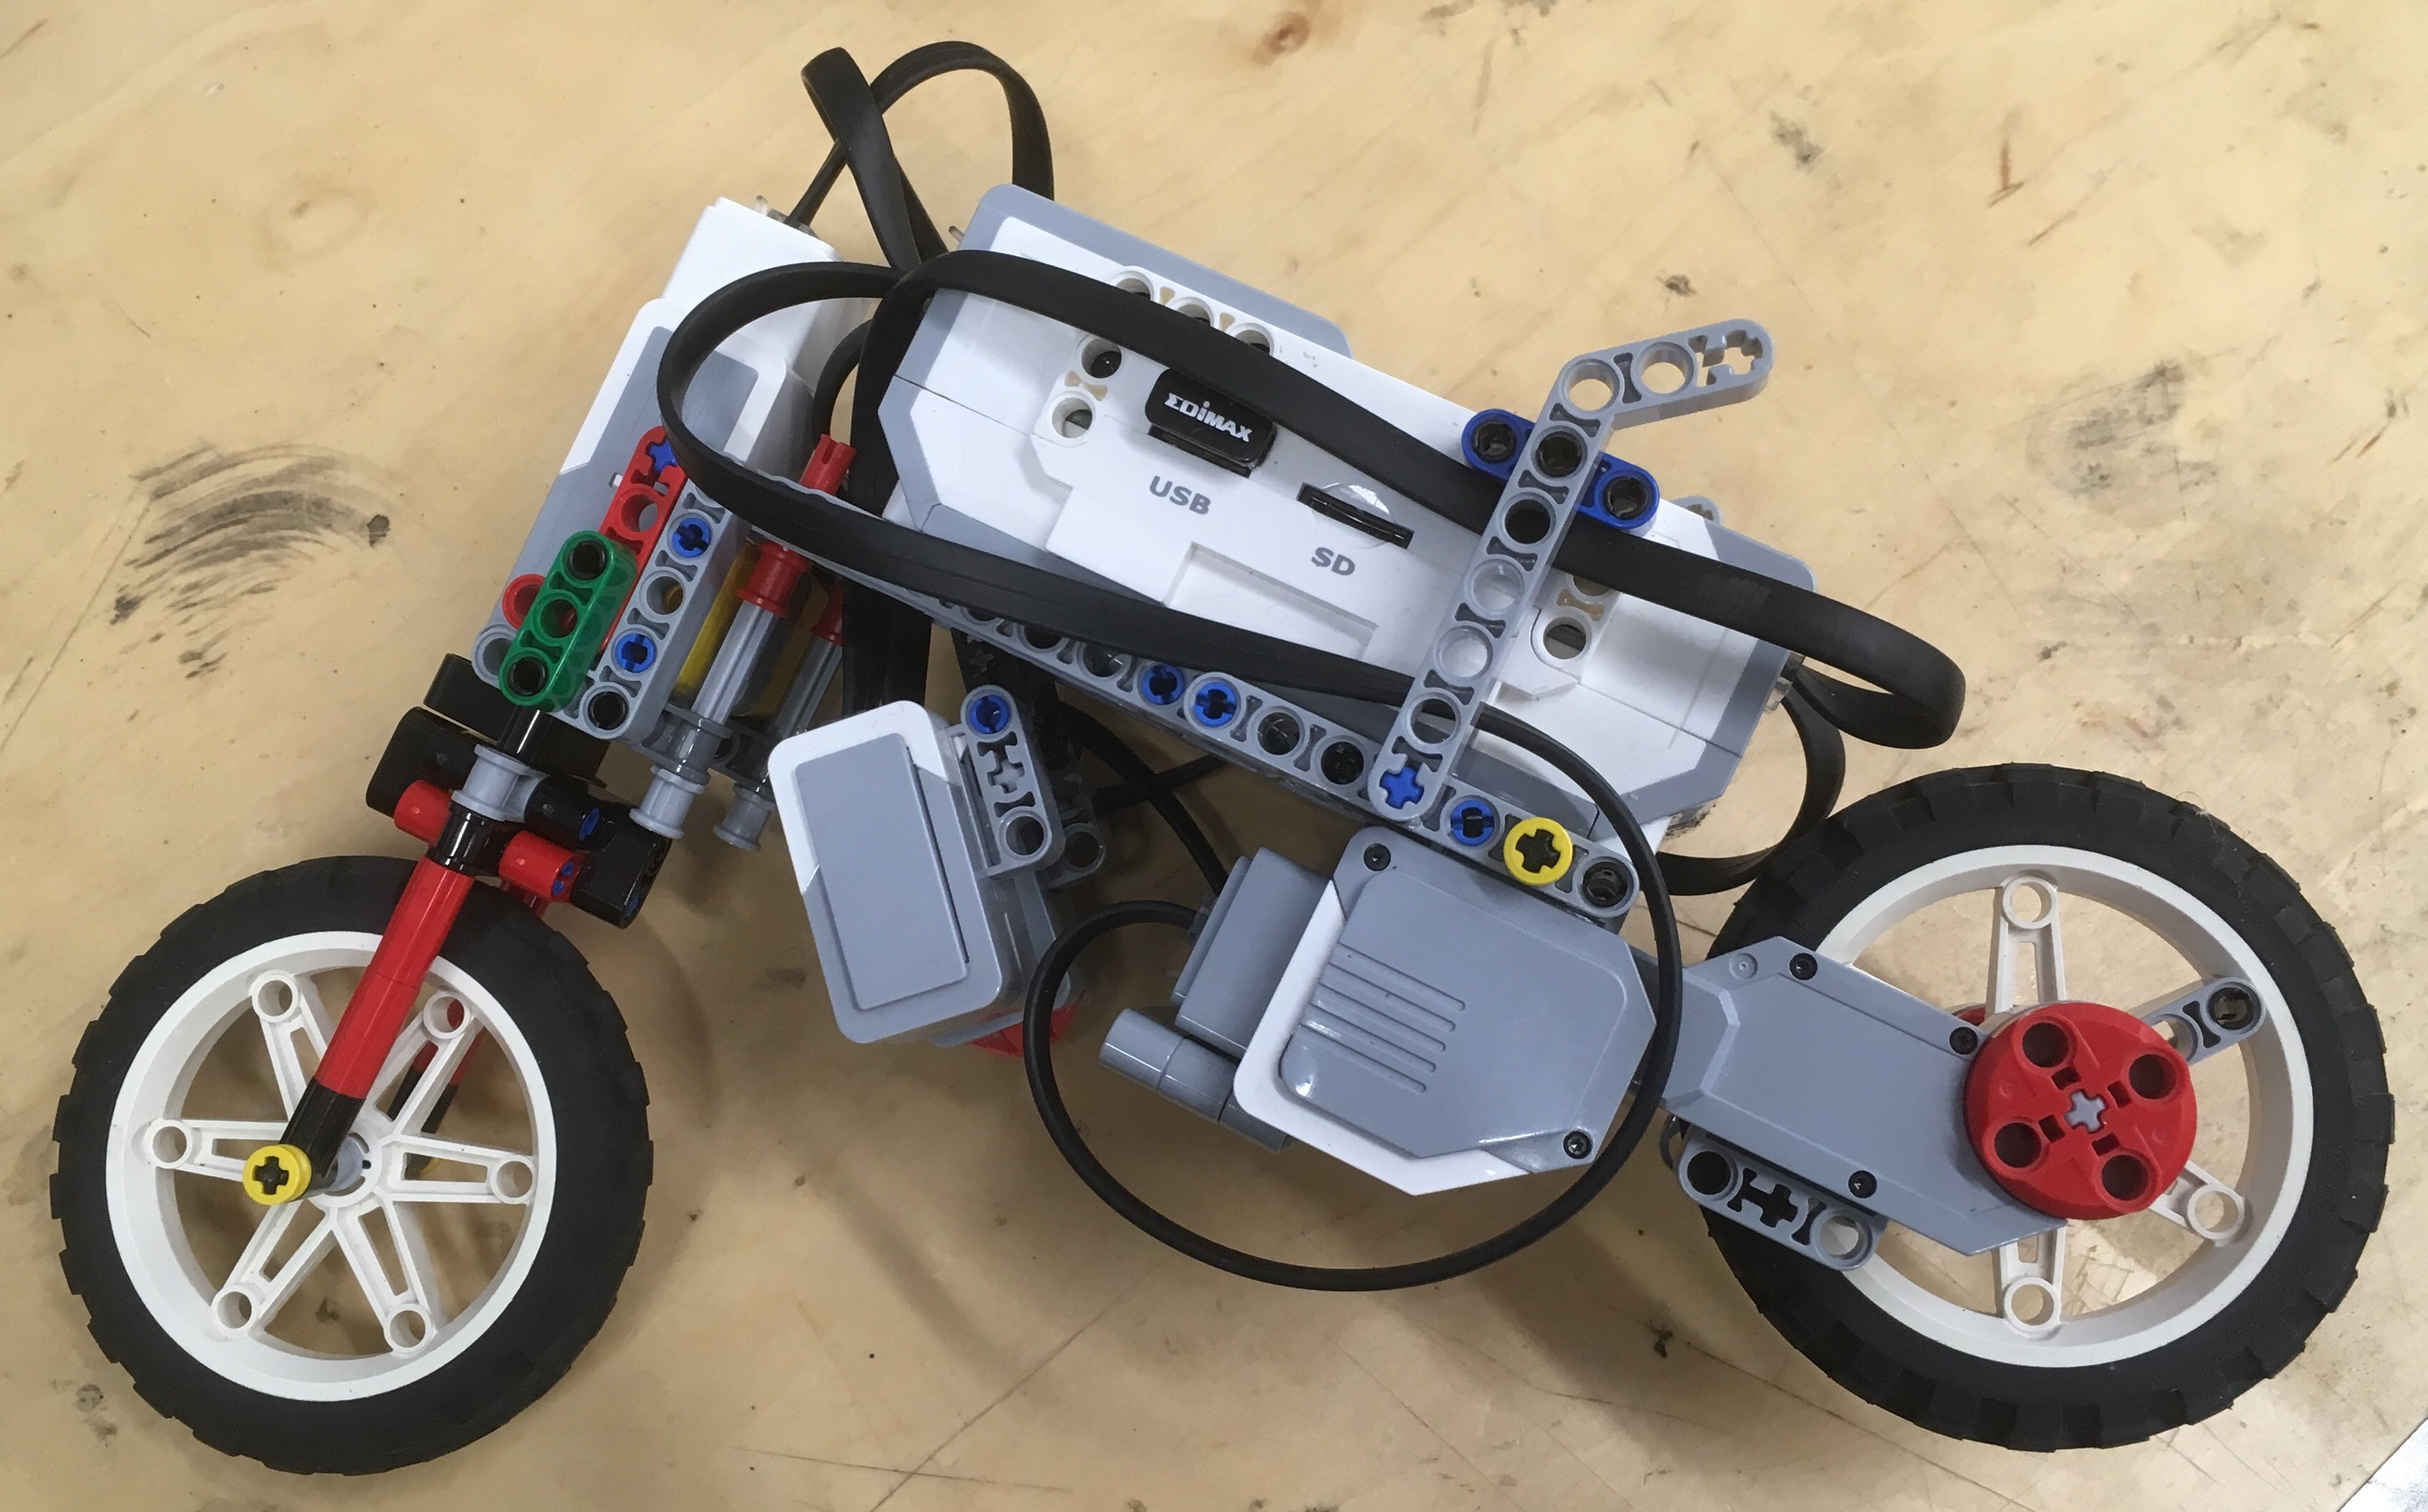
\includegraphics[scale=0.075]{LegoBike.jpg}
\caption{Lego Prototype Bicycle}
\label{fig:lego}
\end{figure}

\subsection{Hardware}
The Lego prototype was made up of standard \textit{Lego Mindstorms EV3} parts. In particular, two large motors are used in parallel to propel the bicycle forwards at a maximum possible speed, whilst a smaller motor was placed at the handlebars to actuate the front fork assembly. Only a single gyroscopic sensor was available to provide a measurement of the rate of change of the lean angle. Lastly, the \textit{Lego EV3 Brick} served as the central processing system, with a 300 MHz ARM processor, 16MB of Flash memory, and 64MB of RAM.

\subsection{Software}
The microprocessor was programmed using RobotC, a C-derivative specifically for Lego systems. The software structure is outlined in pseudo-code below.

\begin{lstlisting}[language=C, caption=Lego Software Pseudo-Code]
initialiseSensorsAndMotors();
bias = calibrateGyroscope();
startDriveMotors(maxSpeed);
startTimer();

while (true) {
	if (currentSampleTime >= desiredSampleTime) {
		leandot = getSensorMeasurement() - bias;
		lean = estimateLeanAngle(leandot);
		ctrl = computeControllerOutput(0.0 - lean);
		pos = actuateHandlebarMotor(ctrl);
		logData(time,lean,ctrl,pos);
	}
}
\end{lstlisting}

The calibration routine records a fixed number of measurements and calculates their mean. This mean bias is then subtracted from each subsequent measurement in the control loop. The controller function computes the output of a difference equation obtained via discretisation, as mentioned in the previous section. Logging of data was achieved via Bluetooth using RobotC's inbuilt logging functionality. Finally, the desired sample time was chosen to be $T=0.01s$.

\subsubsection{Lean Angle Estimation}
The Lego bicycle is only equipped with a gyroscopic sensor, meaning that only the rate of change of the lean angle is directly measurable. Direct integration of this measurement to give an estimate of the lean angle is not possible, since the measurements are corrupted by noise and the gyro has a time-varying bias. This noise and gyro bias will cause a drift in the estimated lean angle over time and thus deviate quickly from the true lean angle. \\

Therefore, it is necessary to estimate the lean angle at every timestep using a continuous-discrete \textit{Extended Kalman Filter} (EKF). The EKF fuses the approximately-known, linearised, continuous system dynamics with discrete, noisy sensor readings to give an overall improved state estimate. Th full derivation of the EKF is given in \cite{smalluav}. The state vector and model dynamics are taken from the second-order model given in section \ref{SecondOrder}. Note that this entire state estimation step would not be necessary if an accelerometer were available, which could be used as reference to correct for drift. \\

The continuous-discrete EKF can be divided into two steps. Firstly, the \textit{prediction} step uses the system dynamics to estimate the state vector a timestep $T$ in the future:
\begin{align*}
\hat{\underline{x}} &= \hat{\underline{x}} + T \cdot \mathbf{A} \\
\mathbf{P} &= \mathbf{P} + T \cdot (\mathbf{A P} + \mathbf{P} \mathbf{A}^T + \mathbf{Q})
\end{align*}

Where $\hat{\underline{x}}$ is the state estimate vector, $\mathbf{A}$ is the linearised state-transition matrix, $\mathbf{P}$ is the error covariance matrix, and $\mathbf{Q}$ is the model noise matrix. \\

Following this, the \textit{update} step fuses the linearised dynamics with the noisy sensor readings:
\begin{align*}
\mathbf{K} &= \mathbf{P} \mathbf{C}^T (\mathbf{R} + \mathbf{C} \mathbf{P} \mathbf{C}^T)^{-1} \\
\mathbf{P} &= (\mathbf{I} - \mathbf{K C}) \mathbf{P} \\
\hat{\underline{x}} &= \hat{\underline{x}} + \mathbf{K} (\underline{y}_m - \mathbf{C} \hat{\underline{x}})
\end{align*}

Where $\underline{y}_m$ is the measurement vector, $\mathbf{C}$ is the state output matrix, $\mathbf{R}$ is the measurement noise matrix, and $\mathbf{K}$ is the Kalman gain, which places a weighting on the measurements and internal model predictions. \\
$\mathbf{Q}$ is chosen depending on the model accuracy, whereas $\mathbf{R}$ is set to the noise covariance found in the sensor datasheet. \\

Lastly, it is important to note that an approximate model of the dynamics is used in conjunction with a noisy, biased sensor. Even though the resulting state estimation performance is much improved over using only the gyroscope readings, the inevitable inaccuracies will accumulate and degrade the lean angle estimate as time progresses. This ultimately has a direct impact on control performance and also only allows the final system to be tested for short periods of time before requiring a reset. \\

This is displayed in the simulated EKF state estimation in Figure \ref{fig:LegoKalman} below, where it is evident that after an initially good estimation performance, after a brief amount of time the lean angle estimate starts to drift away from the true value.

\begin{figure}[H]
	\centering
	\begin{tikzpicture}
		\begin{axis}
			[xlabel=Time (s),
			 ylabel=Lean Angle $\phi$ (deg),
			 xmin=0,xmax=4.0,
			 ymin=-1,ymax=1.5,
			 legend pos=north east,
			 tick label style={/pgf/number format/fixed}]
			\addplot[mark=none,dashed] table[x=t,y=true,col sep=comma] {legoKalman.csv};	
			\addplot[mark=none,color=blue] table[x=t,y=estimate,col sep=comma] {legoKalman.csv};
			\legend{True,Model}
		\end{axis}
	\end{tikzpicture}
	\caption{EKF Lean Angle Estimation}
	\label{fig:LegoKalman}
\end{figure}

\subsection{Results}

\subsubsection{PID}
A proportional-only controller was indeed able to stabilise the bicycle. As predicted by the second-order model and simulation, the bicycle could be stabilised at the given forward speed of $V=0.44ms^{-1}$ by a gain greater than 11.4. \\
Figures \ref{fig:LegoPController} a) and b) show an excerpt of the response and controller effort of the Lego prototype for a proportional gain of $K_P=12$.

\begin{figure}[H]
	\begin{subfigure}{0.5\textwidth}
	\begin{tikzpicture}
		\begin{axis}
			[xlabel=Time (s),
			 ylabel=Lean Angle $\phi$ (deg),			 
			 xmin=0,xmax=4,
			 ymin=-8,ymax=8,
			 tick label style={/pgf/number format/fixed}]
			\addplot[mark=none] table[x=t,y=phi, col sep=comma] {legoP12.csv};		
		\end{axis}
	\end{tikzpicture}
	\caption{Lean Angle Response}
	\end{subfigure} \hspace{1mm}
	\begin{subfigure}{0.5\textwidth}
	\begin{tikzpicture}
		\begin{axis}
			[xlabel=Time (s),
			 ylabel=Steering Angle $\delta$ (deg),
			 xmin=0,xmax=4,
			 ymin=-75,ymax=75,
			 legend pos=north west,
			 tick label style={/pgf/number format/fixed}]
			\addplot[mark=none,color=red] table[x=t,y=delta, col sep=comma] {legoP12.csv};			
		\end{axis}
	\end{tikzpicture}
	\caption{Actuator Effort}
	\end{subfigure}
	\caption{P-Controller Response ($K_P=12$)}
	\label{fig:LegoPController}
\end{figure}

The response for the simple proportional controller is certainly not ideal, even though stability is achieved.  The magnitude of the lean angle is bounded by approximately $5^{\circ}$, which is an acceptable deviation from the desired setpoint of $0^{\circ}$. However, there is an oscillation present in the response, indicating that the system is on the boundary of stability. Knocking the bicycle gently, as to add an output disturbance, destabilises it. Thus the closed-loop system is not robust and sensitive to disturbances in its current state. This is to be expected however, since we are using a proportional gain which places the closed-loop poles very close to the imaginary axis. As shown, inevitable model uncertainties will deteriorate the control performance from the ideal calculations and simulations. Furthermore, this \textit{jittering} behaviour also causes the bicycle to move off-track easily and not follow a straight path. Lastly, the controller effort is larger than ideal. However, this large actuator command is required for stability. \\

As a brief aside, the servo model is again verified by running a simulation in Matlab but using the real-world controller output data. As can be seen in Figure \ref{fig:LegoServoIDPart2}, the match is near perfect and confirms the actuator model identified in an earlier section of this report. \\

\begin{figure}[H]
\centering
\begin{tikzpicture}
		\begin{axis}
			[xlabel=Time (s),
			 ylabel=Steering Angle $\delta$ (deg),
			 xmin=0,xmax=4,
			 ymin=-75,ymax=75,
			 legend pos=north west,
			 tick label style={/pgf/number format/fixed}]
			\addplot[mark=none,dashed] table[x=t,y=delta, col sep=comma] {legoP12.csv};
			\addplot[mark=none,color=blue] table[x=t, y=deltasim, col sep=comma] {legoP12.csv};
		\end{axis}
	\end{tikzpicture}
	\caption{Lego Servo Model Verification}
	\label{fig:LegoServoIDPart2}
\end{figure}

\subsubsection{LQR}

\subsubsection{$H_{\infty}$ Loop-Shaping}

\subsubsection{Final Observations}
hard to stabilise since h is small and time constants are short, not robust to disturbances. Have hardly any time to react. Additional limitation is maximum speed of lego model, which causes it to be very unstable. Stabilisation can be achieved but not a very good performance. Performance could probably be improved if we were to use a better angle estimation system, i.e. use an IMU. As soon as gyro estimate starts drifting we're in trouble (which turns out to be pretty quickly)...